\section{Análisis}

Usando \textit{Gephi}, se han obtenido algunas medidas básicas de la red, las
cuales se pueden ver en el cuadro~\ref{tab:measurements}. Fijándonos en estas
medidas, lo primero que destacamos es que la densidad del grafo es muy baja, lo
cual ya intuíamos por el anillo de nodos aislados del que hablábamos en la
figura~\ref{fig:network-parties}. Esto también se refleja en la medida del
número de nodos y de aristas que contiene la componente gigante, ya que se
"pierden" el 17.99\% de los nodos pero se mantienen casi el 100\% de las
aristas.

\begin{table}[h!]
    \caption{Medidas obtenidas de la red}
    \label{tab:measurements}
    \begin{center}
    \begin{tabular}{ |c|c| }
        \hline
        \textbf{Medida} & \textbf{Valor} \\
        \hline
        Número de nodos $N$ & 1490 \\
        \hline
        Número de enlaces $L$ & 19025 \\
        \hline
        Número máximo de enlaces $L_{max}$ & 2113889 \\
        \hline
        Densidad del grafo $L/L_{max}$ & 0.009 \\
        \hline
        Grado medio $\langle k \rangle$ & 12.768 \\
        \hline
        Diámetro $d_{max}$ & 9 \\
        \hline
        Distancia media $d$ & 3.3902 \\
        \hline
        Coeficiente medio de \textit{clustering} $\langle C \rangle$ & 0.172 \\
        \hline
        Número de componentes conexas & 268 \\
        \hline
        Número de nodos componente gigante (y \%) & 1222 (82.01\%) \\
        \hline
        Número de aristas componente gigante (y \%) & 19024 (99.99\%) \\
        \hline
    \end{tabular}
    \end{center}
\end{table}

En la figura~\ref{fig:degree-distribution} vemos la distribución del grado de la
red, es decir, del número de enlaces que conectan cada nodo con otros. Tenemos 4
\textit{hubs} que tienen más de 350 enlaces, pero el 56.31\% de los nodos no
tienen más de 12 enlaces (el grado medio es de 12.768).

Al tratarse de un grafo dirigido, vamos a fijarnos también en las distribuciones
del prestigio de entrada y de salida, representadas en las figuras
\ref{fig:indegree-distribution} y \ref{fig:outdegree-distribution},
respectivamente. Mientras que solo hay un nodo que realiza referencias a más de
250 blogs, tenemos hasta 9 nodos a los que llegan enlaces de más de 200.
Entendemos entonces que hay unos pocos blogs más importantes o conocidos a los
que enlazan muchos otros blogs más pequeños.

\begin{figure}
    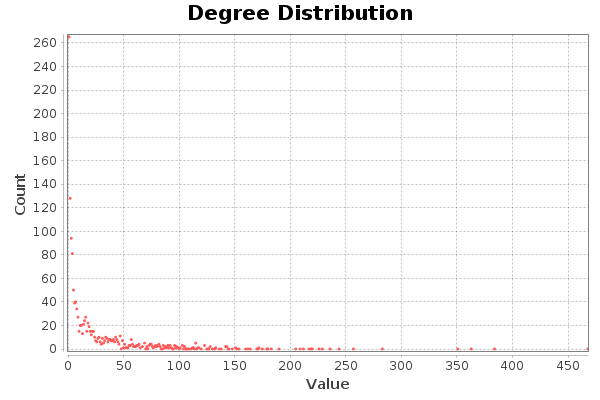
\includegraphics[width=\textwidth]{images/plots/degree-distribution.png}
    \caption{Distribución del grado}
    \label{fig:degree-distribution}
\end{figure}

\begin{figure}
    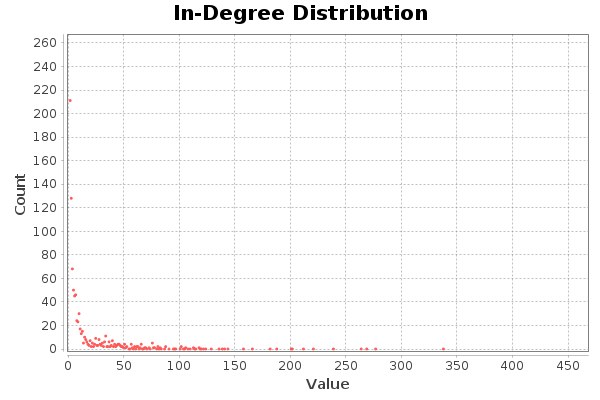
\includegraphics[width=\textwidth]{images/plots/indegree-distribution.png}
    \caption{Distribución del prestigio de entrada}
    \label{fig:indegree-distribution}
\end{figure}

\begin{figure}
    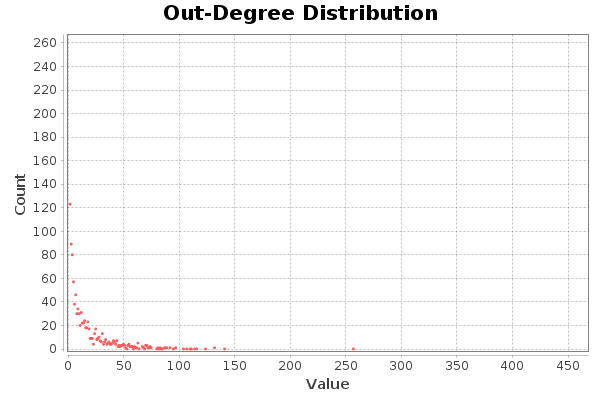
\includegraphics[width=\textwidth]{images/plots/outdegree-distribution.png}
    \caption{Distribución del prestigio de salida}
    \label{fig:outdegree-distribution}
\end{figure}

\newpage

Volviendo a fijarnos en el cuadro~\ref{tab:measurements}, vemos como la red
tiene diámetro 9, mientras que la distancia media de los caminos es de 3.3902.
Calculando esta medida, también hemos obtenido distribuciones relativas a las
distintas medidas de cercanía, que se pueden ver en las figuras
\ref{fig:closeness-centrality-distribution} a
\ref{fig:eccentricity-distribution}. Todas estas medidas han sido normalizadas.

En la distribución de la intermediación
(figura~\ref{fig:betweenness-centrality-distribution}), nos encontramos con
valores muy bajos, por lo que no tenemos ningún nodo concreto que actue como
puente o portero entre grupos de nodos.

En cuanto a la cercanía (figura~\ref{fig:closeness-centrality-distribution}), sí
que tenemos algunos nodos con un valor muy alto, es decir, que se encuentran en
una posición muy céntrica dentro de la red.

\begin{figure}
    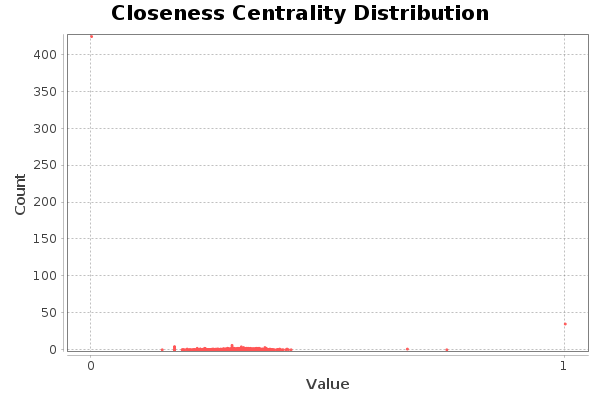
\includegraphics[width=\textwidth]{images/plots/closeness-centrality-distribution.png}
    \caption{Distribución de la centralidad de cercanía}
    \label{fig:closeness-centrality-distribution}
\end{figure}

\begin{figure}
    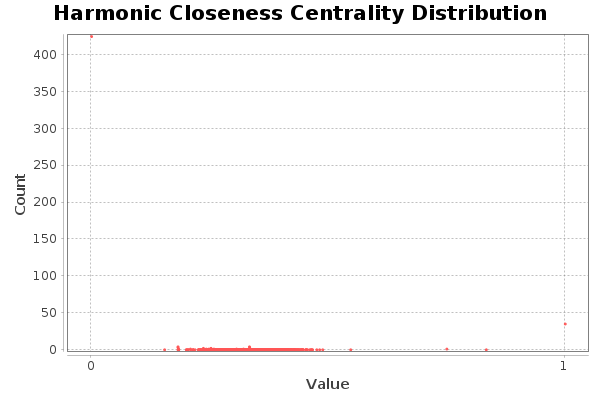
\includegraphics[width=\textwidth]{images/plots/harmonic-closeness-centrality-distribution.png}
    \caption{Distribución de la centralidad armónica de cercanía}
    \label{fig:harmonic-closeness-centrality-distribution}
\end{figure}

\begin{figure}
    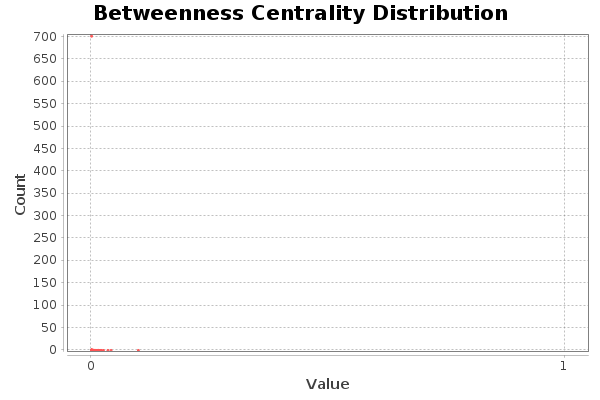
\includegraphics[width=\textwidth]{images/plots/betweenness-centrality-distribution.png}
    \caption{Distribución de la centralidad de intermediación}
    \label{fig:betweenness-centrality-distribution}
\end{figure}

\begin{figure}
    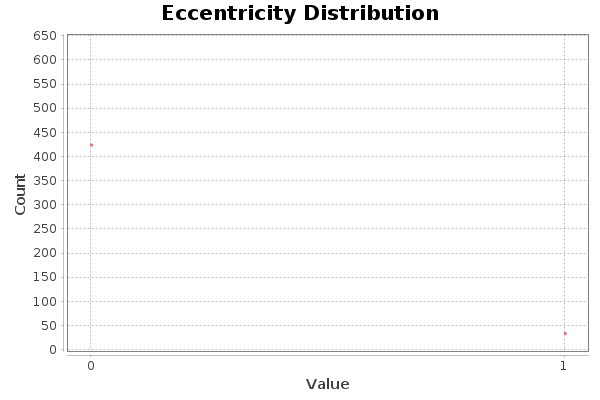
\includegraphics[width=\textwidth]{images/plots/eccentricity-distribution.png}
    \caption{Distribución de la excentricidad}
    \label{fig:eccentricity-distribution}
\end{figure}

\newpage

En cuanto a la conectividad, tenemos 268 componentes conexas, muchas de ellas
presentes en el "cinturón" de nodos aislados del que hemos hablado en la
figura~\ref{fig:network-parties}.

El coeficiente de clustering, cuya distribución tenemos en la
figura~\ref{fig:clustering-distribution}, tiene un valor medio de 0.172, lo que
es bastante bajo. En la distribución vemos que la mayoría de nodos tienen un
valor de este coeficiente inferior a 0.5. Esto puede deberse a que, como ya
hemos visto, la red es muy poco densa.

\begin{figure}
    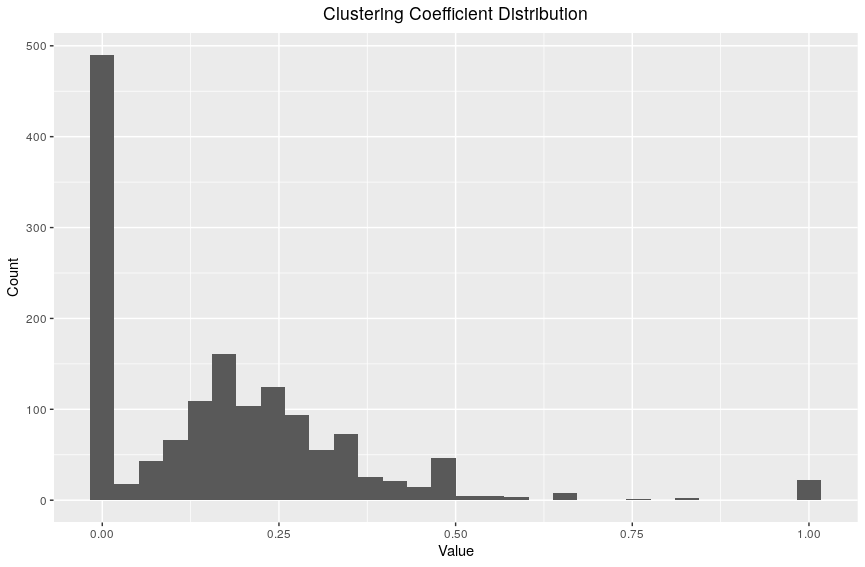
\includegraphics[width=\textwidth]{images/plots/clustering-coefficient-distribution.png}
    \caption{Distribución del coeficiente de \textit{clustering}}
    \label{fig:clustering-distribution}
\end{figure}
